% !TeX root = ../main.tex
\section{Giới thiệu}

\subsection{Mục tiêu của bài báo cáo}

Trong những năm gần đây, học sâu (deep learning) đã trở thành một trong những hướng tiếp cận quan trọng và hiệu quả nhất trong lĩnh vực thị giác máy tính (computer vision). Nhờ khả năng tự động học đặc trưng từ dữ liệu, các mô hình học sâu đã đạt được những kết quả vượt trội trong nhiều bài toán như phân loại ảnh, phát hiện đối tượng và nhận dạng khuôn mặt. Đặc biệt, sự phát triển của các kiến trúc hiện đại như Convolutional Neural Networks (CNN) \cite{vaswani2017attention} và Vision Transformer (ViT) \cite{dosovitskiy2020image} đã mở ra nhiều hướng nghiên cứu và ứng dụng mới.

Bài báo cáo này tập trung vào bài toán phân loại ảnh, một trong những bài toán cơ bản nhưng mang tính nền tảng trong thị giác máy tính. Mục tiêu chính là xây dựng, huấn luyện và so sánh hiệu năng của nhiều mô hình học sâu khác nhau, từ các mô hình đơn giản như \textbf{Softmax Regression} và \textbf{Multi-Layer Perceptron (MLP)} đến các mô hình phức tạp hơn như \textbf{CNN} và \textbf{Vision Transformer}. Thông qua đó, người thực hiện có thể hiểu rõ hơn về cách các mô hình học được biểu diễn dữ liệu ảnh cũng như ưu, nhược điểm của từng kiến trúc.

Bên cạnh việc sử dụng các thành phần có sẵn trong thư viện PyTorch \cite{paszke2019pytorch}, báo cáo còn đi sâu vào việc tự hiện thực một số thành phần quan trọng, điển hình là khối Transformer Encoder. Điều này giúp làm rõ cơ chế hoạt động bên trong của mô hình Transformer, từ đó nâng cao khả năng hiểu và tùy biến mô hình cho các bài toán thực tế.

Ngoài ra, báo cáo cũng khảo sát các hướng mở rộng như kết hợp nhiều kiến trúc khác nhau (ví dụ CNN kết hợp Transformer), các phương pháp biểu diễn ảnh đa dạng, cũng như áp dụng các mô hình chuỗi như LSTM \cite{vennerod2021lstm}, GRU \cite{chung2014empirical} cho dữ liệu ảnh. Những thử nghiệm này nhằm mục đích khám phá sâu hơn không gian thiết kế mô hình và đánh giá ảnh hưởng của từng lựa chọn đến hiệu năng tổng thể.

Thông qua quá trình thực nghiệm và phân tích, báo cáo hướng đến việc cung cấp một cái nhìn toàn diện về các phương pháp tiếp cận khác nhau trong bài toán phân loại ảnh, đồng thời rút ra những nhận xét và bài học quan trọng trong việc xây dựng và đánh giá mô hình học sâu.

\subsection{Giới thiệu về tập dữ liệu CIFAR-10}

Trong bài báo cáo này, nhóm sử dụng tập dữ liệu \textbf{CIFAR-10} \cite{krizhevsky2009learning} để thực hiện các thí nghiệm phân loại ảnh. CIFAR-10 là một trong những tập dữ liệu phổ biến và tiêu chuẩn trong lĩnh vực thị giác máy tính, thường được sử dụng để đánh giá hiệu năng của các mô hình học máy và học sâu.

\subsubsection{Lý do lựa chọn CIFAR-10}

Việc lựa chọn CIFAR-10 cho bài toán này dựa trên một số lý do chính sau:

\begin{itemize}
\item \textbf{Phù hợp với mục tiêu bài tập:} CIFAR-10 có độ phức tạp vừa phải, đủ để thể hiện sự khác biệt giữa các mô hình như MLP, CNN và Transformer, nhưng vẫn có thể huấn luyện trong thời gian hợp lý.
\item \textbf{Dữ liệu chuẩn và phổ biến:} Đây là benchmark phổ biến, giúp dễ dàng so sánh kết quả với các nghiên cứu và triển khai trước đó.
\item \textbf{Kích thước nhỏ gọn:} Ảnh có kích thước nhỏ giúp giảm chi phí tính toán, phù hợp với môi trường thực nghiệm hạn chế tài nguyên.
\item \textbf{Đa dạng về đặc trưng hình ảnh:} Bao gồm nhiều loại đối tượng với đặc trưng khác nhau (động vật, phương tiện), giúp đánh giá khả năng trích xuất đặc trưng của mô hình.
\end{itemize}

Ngoài ra, theo quan sát từ quá trình thực nghiệm của nhóm, CIFAR-10 cũng cho thấy sự khác biệt rõ ràng về hiệu năng giữa các kiến trúc mô hình, từ đó giúp việc phân tích và so sánh trở nên trực quan và có ý nghĩa hơn.

\subsubsection{Đặc trưng của dữ liệu hình ảnh}

CIFAR-10 là tập dữ liệu gồm tổng cộng \textbf{60,000 ảnh màu}, mỗi ảnh có kích thước nhỏ $32 \times 32$ pixel. Tập dữ liệu được chia thành \textbf{10 lớp đối tượng}, bao gồm: airplane, automobile, bird, cat, deer, dog, frog, horse, ship, truck.

Về cách phân chia dữ liệu:
\begin{itemize}
\item \textbf{50,000 ảnh} được sử dụng cho tập huấn luyện (training set)
\item \textbf{10,000 ảnh} còn lại được dùng cho tập kiểm tra (test set)
\end{itemize}

Đặc điểm nổi bật của CIFAR-10 là kích thước ảnh nhỏ nhưng chứa nhiều biến thể về góc nhìn, ánh sáng và nền, khiến bài toán phân loại trở nên không hề đơn giản. Điều này giúp tập dữ liệu trở thành một lựa chọn phù hợp để đánh giá khả năng học đặc trưng của các mô hình từ cơ bản đến nâng cao.

\subsubsection{Phân phối dữ liệu}

Phân phối số lượng mẫu theo từng lớp trong tập huấn luyện CIFAR-10 được minh họa trong Hình~\ref{fig:cifar10_distribution}. 

\begin{figure}[H]
\centering
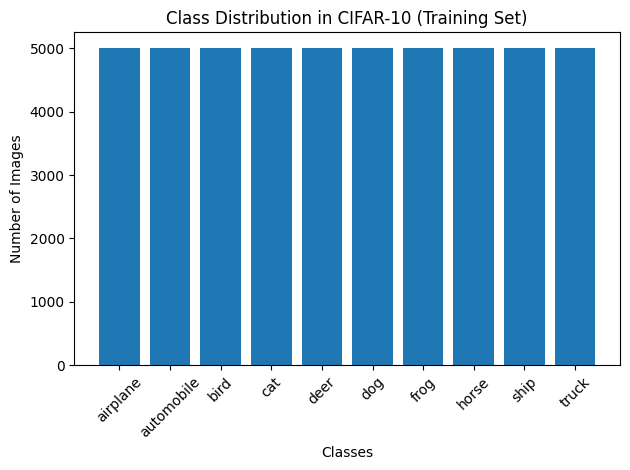
\includegraphics[width=0.7\linewidth]{images/class_distribution_cifar10.png}
\caption{Class distribution of the CIFAR-10 training dataset}
\label{fig:cifar10_distribution}
\end{figure}

Như có thể quan sát, tập dữ liệu CIFAR-10 có phân phối hoàn toàn cân bằng, với mỗi lớp chứa khoảng 5,000 ảnh trong tập huấn luyện. Điều này đảm bảo rằng không có lớp nào chiếm ưu thế trong quá trình huấn luyện, từ đó giúp mô hình học được các đặc trưng một cách công bằng giữa các lớp.

Tính cân bằng của dữ liệu giúp giảm thiểu nguy cơ bias trong mô hình và cho phép việc đánh giá hiệu năng trở nên khách quan hơn. Do đó, trong bài toán này, không cần áp dụng các kỹ thuật xử lý mất cân bằng dữ liệu như oversampling hoặc class weighting.

\subsubsection{Trực quan hóa dữ liệu}

Để hiểu rõ hơn về đặc điểm của tập dữ liệu, một số ảnh mẫu từ mỗi lớp trong CIFAR-10 được trực quan hóa như trong Hình~\ref{fig:cifar10_samples}.

\begin{figure}[H]
\centering
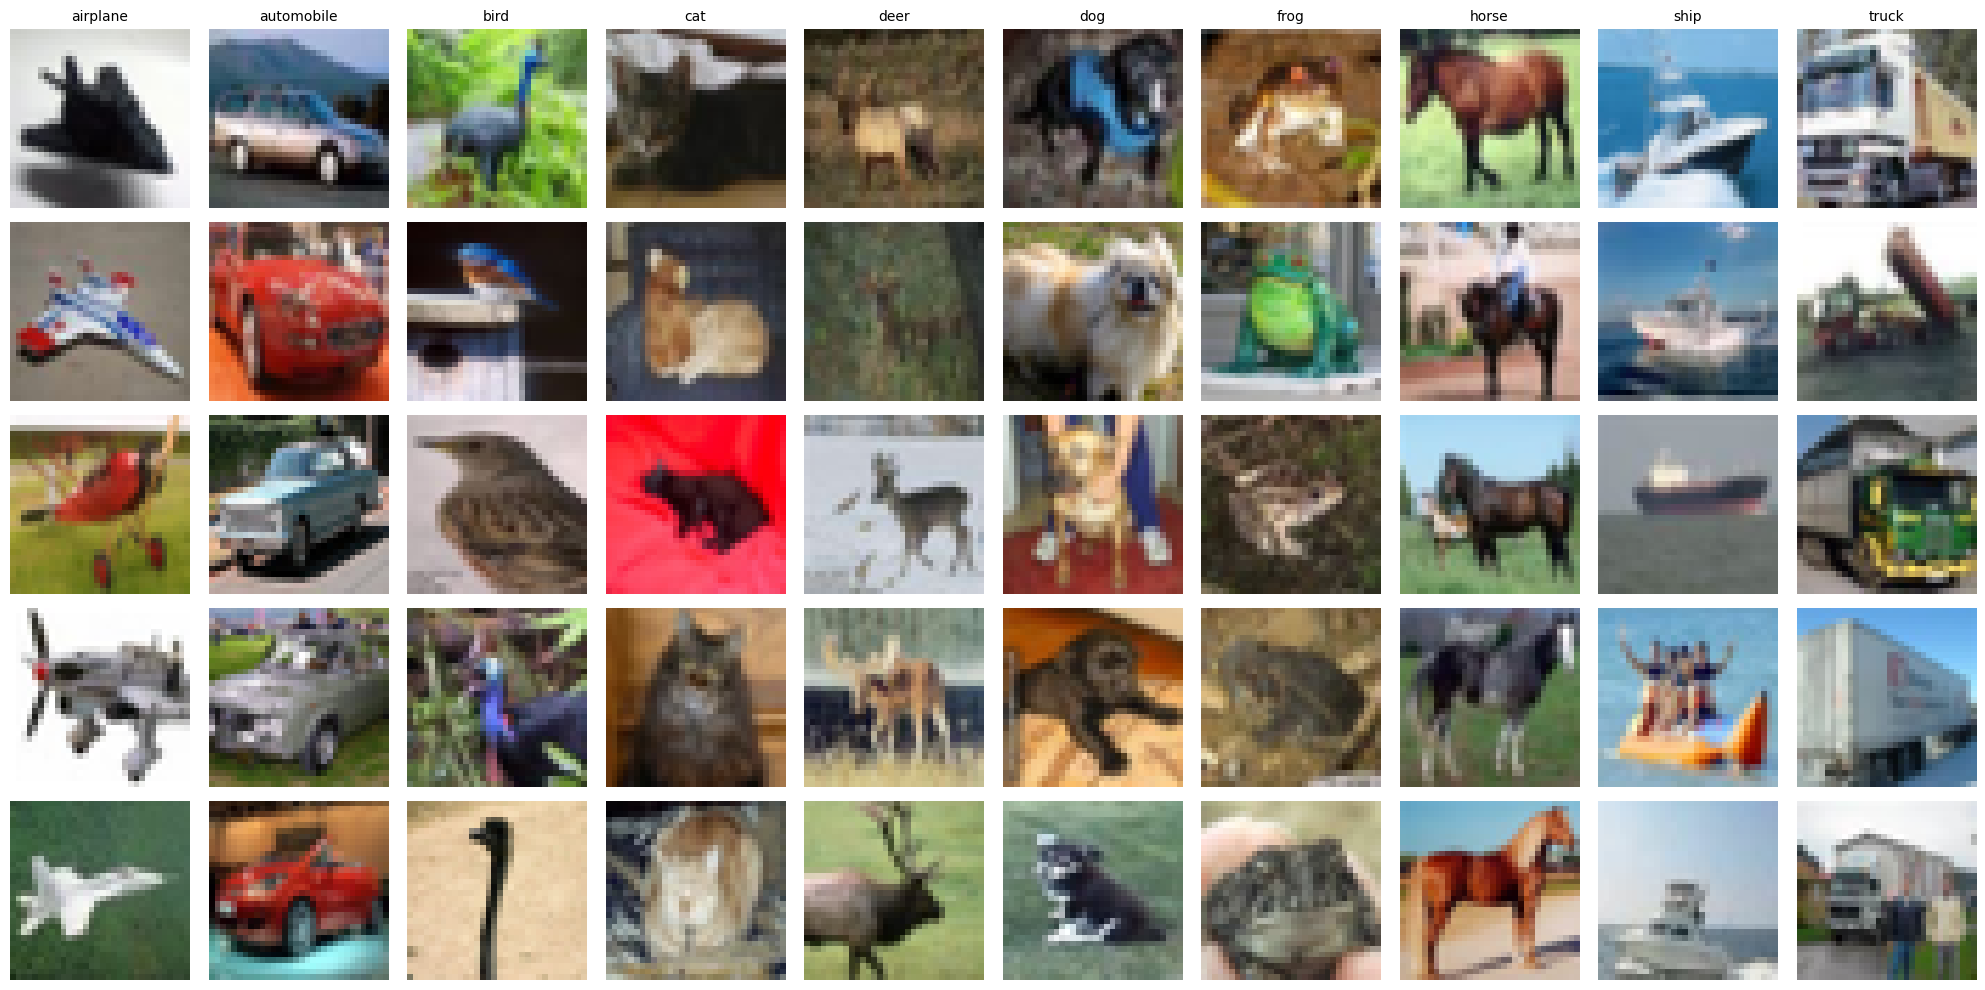
\includegraphics[width=0.9\linewidth]{images/cifar10_samples.png}
\caption{Sample images from each class in CIFAR-10}
\label{fig:cifar10_samples}
\end{figure}

Từ hình trên, có thể nhận thấy rằng các đối tượng trong CIFAR-10 xuất hiện với nhiều biến thể khác nhau về góc nhìn, vị trí và nền. Ngoài ra, các ảnh có độ phân giải thấp (32×32), khiến cho các đặc trưng chi tiết bị hạn chế.

Bên cạnh đó, một số lớp có sự tương đồng về mặt hình ảnh, ví dụ như \textit{cat} và \textit{dog} làm tăng độ khó của bài toán phân loại.

\begin{figure}[H]
\centering
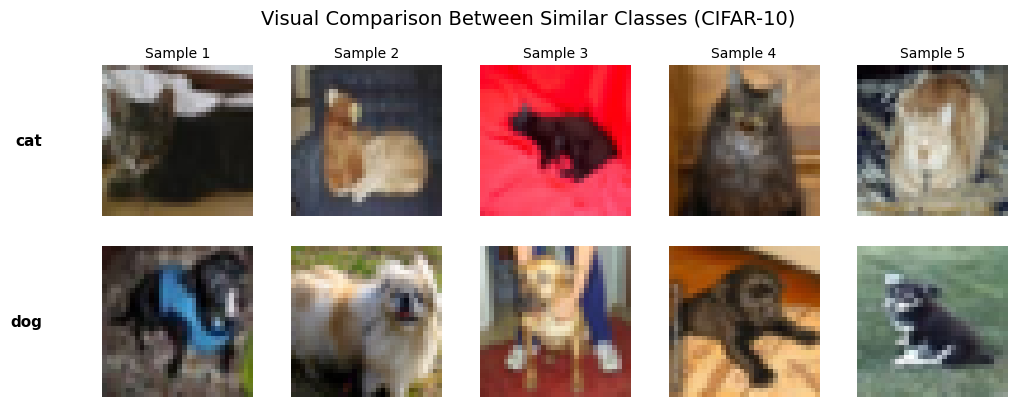
\includegraphics[width=0.9\linewidth]{images/cat_and_dog_visualization.png}
\caption{Sample images from each class in CIFAR-10}
\label{fig:cat_and_dog_visualization}
\end{figure}

Ngoài ra, các ảnh trong CIFAR-10 thường chứa nền đa dạng và phức tạp, trong đó đối tượng chính không phải lúc nào cũng nổi bật hoặc nằm ở vị trí trung tâm. Sự thay đổi về background giữa các ảnh trong cùng một lớp có thể gây nhiễu và làm tăng độ khó trong việc trích xuất đặc trưng.

\begin{figure}[H]
\centering
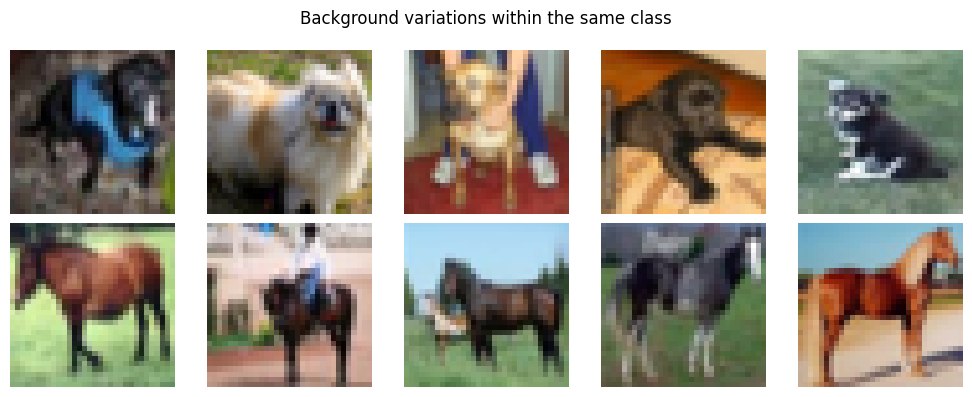
\includegraphics[width=0.9\linewidth]{images/background_variantions.png}
\caption{Examples of background variations within the same class}
\label{fig:background_variations}
\end{figure}

Những đặc điểm này cho thấy rằng mô hình cần có khả năng trích xuất đặc trưng không gian một cách hiệu quả, đồng thời phải đủ mạnh để xử lý sự biến thiên lớn về hình dạng, vị trí và điều kiện nền của đối tượng. 

Cụ thể, mô hình cần học được các biểu diễn mang tính bất biến (invariant) đối với các thay đổi về góc nhìn, tỉ lệ và ánh sáng, đồng thời vẫn phân biệt được các lớp có đặc điểm hình ảnh tương đồng. 

Do đó, các kiến trúc có khả năng khai thác cấu trúc không gian của ảnh, chẳng hạn như các mô hình học sâu dựa trên tích chập hoặc attention, được kỳ vọng sẽ đạt hiệu năng tốt hơn trên tập dữ liệu này.